\begin{figure}
\centering
\begin{subfigure}{0.45\textwidth}
\includemedia[width=\textwidth,activate=onclick,addresource=images/animations/ri_lownoise.mp4,flashvars={source=images/animations/ri_lownoise.mp4&loop=true&autoPlay=true}]{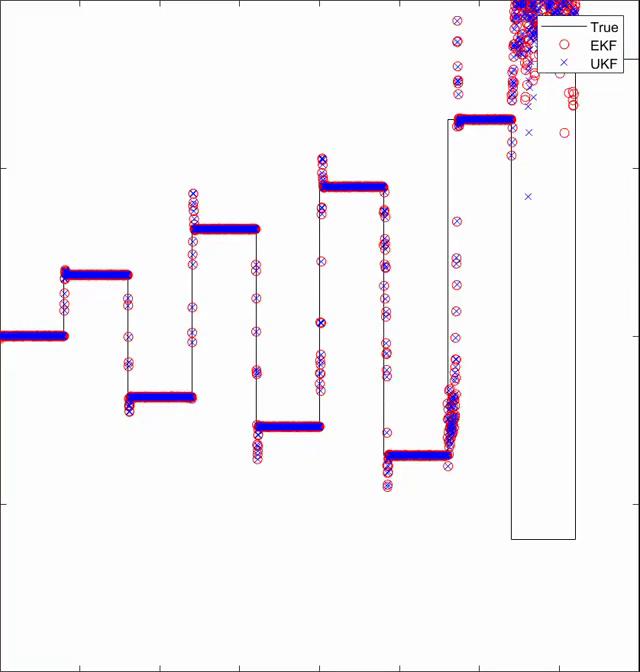
\includegraphics[width=\textwidth]{images/animations/ri_lownoise_thumb.png}}{VPlayer.swf}
\caption{SNR $34\si{\decibel}$, $\sigma_{\omega,\text{noise}}=0$}
\label{fig:ri_lownoise_anim}
\end{subfigure}
\quad
\begin{subfigure}{0.45\textwidth}
\includemedia[
width=\textwidth,activate=onclick,addresource=images/animations/ri_highnoise.mp4,flashvars={
source=images/animations/ri_highnoise.mp4&loop=true&autoPlay=true}]{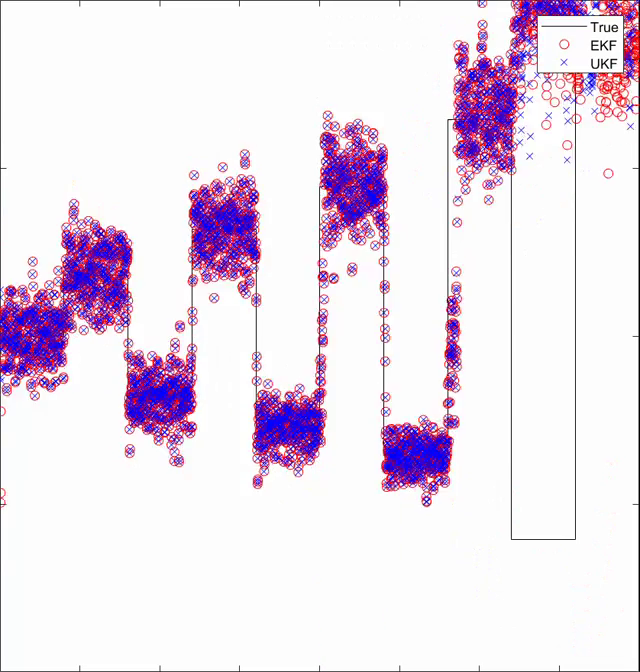
\includegraphics[width=\textwidth]{images/animations/ri_highnoise_thumb.png}}{VPlayer.swf}
\caption{SNR $8\si{\decibel}$, $\sigma_{\omega,\text{noise}}=30\%$}
\label{fig:ri_highnoise_anim}
\end{subfigure}

\caption{Visualization of some predictions for the computation of the RI index with $\sigma=\num{1e+1}$, $q=\num{1e-5}$}
\label{fig:ri_animation}
\end{figure}